\documentclass[tikz,border=2pt]{standalone}
% Preámbulo común de los diagramas TikZ (misma paleta y letra que las notas)
\usepackage[T1]{fontenc}\usepackage[utf8]{inputenc}
\usepackage{libertinus}\usepackage{libertinust1math}
\usepackage[defaultsans,scale=0.92]{lato}
\usepackage{amsmath,amssymb,bm}
\usepackage{tikz}\usetikzlibrary{calc,positioning,arrows.meta,shapes.geometric,decorations.pathreplacing,decorations.pathmorphing,fit,backgrounds}
\definecolor{snlazul}{HTML}{1E5AA8}\definecolor{snlnoche}{HTML}{14213D}\definecolor{snlvioleta}{HTML}{6C4AB6}
\definecolor{snlcoral}{HTML}{D1495B}\definecolor{snlambar}{HTML}{E09F3E}\definecolor{snlverde}{HTML}{2A9D8F}
\definecolor{snlteal}{HTML}{0F7173}\definecolor{snlgris}{HTML}{5C677D}\definecolor{snlfondo}{HTML}{F4F6FA}
\tikzset{>={Stealth[length=2.2mm]},
  bloque/.style={draw=#1,fill=#1!8,thick,rounded corners=2pt,minimum height=11mm,minimum width=20mm,align=center,font=\small},
  bloque/.default=snlazul,
  suma/.style={draw=snlnoche,thick,circle,inner sep=0pt,minimum size=5mm},
  flecha/.style={->,thick,draw=snlnoche},
  etq/.style={font=\small,text=snlnoche},
  nota/.style={font=\footnotesize\sffamily,text=snlgris,align=center}}

\begin{document}
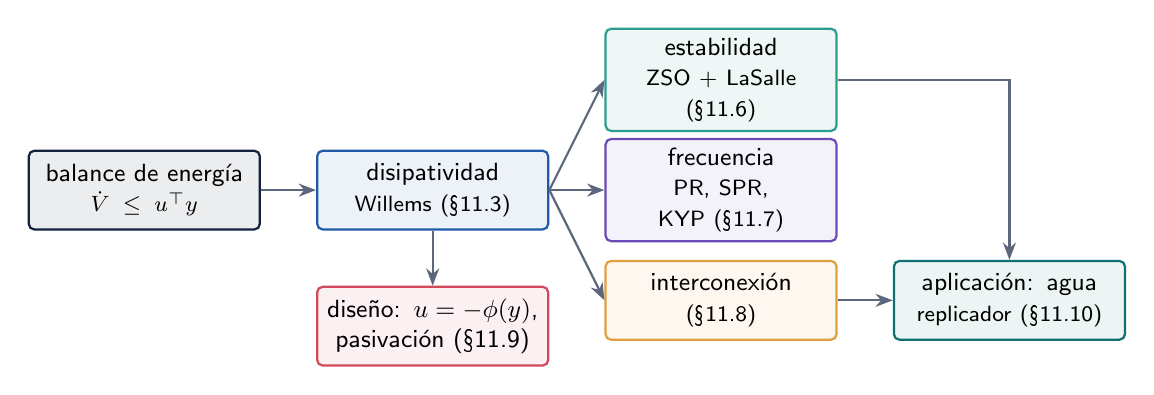
\begin{tikzpicture}[font=\sffamily\small,
  caja/.style={draw=#1,fill=#1!8,thick,rounded corners=2pt,align=center,minimum height=10mm,text width=27mm},
  fl/.style={-{Stealth[length=2.2mm]},thick,draw=snlgris}]
  \node[caja=snlnoche] (bal) {balance de energía\\ \footnotesize $\dot V\le u^\top y$};
  \node[caja=snlazul,right=7mm of bal] (dis) {disipatividad\\ \footnotesize Willems (\S11.3)};
  \node[caja=snlverde,right=7mm of dis,yshift=14mm] (est) {estabilidad\\ \footnotesize ZSO + LaSalle (\S11.6)};
  \node[caja=snlvioleta,right=7mm of dis] (lin) {frecuencia\\ \footnotesize PR, SPR, KYP (\S11.7)};
  \node[caja=snlambar,right=7mm of dis,yshift=-14mm] (int) {interconexión\\ \footnotesize (\S11.8)};
  \node[caja=snlcoral,below=7mm of dis] (dise) {diseño: $u=-\phi(y)$,\\ pasivación (\S11.9)};
  \node[caja=snlteal,right=7mm of int] (agua) {aplicación: agua\\ \footnotesize replicador (\S11.10)};
  \draw[fl] (bal) -- (dis);
  \draw[fl] (dis.east) -- (est.west); \draw[fl] (dis.east) -- (lin.west); \draw[fl] (dis.east) -- (int.west);
  \draw[fl] (dis) -- (dise); \draw[fl] (int) -- (agua); \draw[fl] (est.east) -| (agua.north);
\end{tikzpicture}
\end{document}
